\section{Results}
\label{sec:results}

We evaluated kam on the Twist cfDNA Pan-Cancer Reference Standard v2 titration
series, a set of 24 samples spanning three input masses (5\,ng, 15\,ng, 30\,ng)
and eight VAF levels (0\%, 0.001\%, 0.01\%, 0.1\%, 0.25\%, 0.5\%, 1\%, 2\%).
The truth set contains 375 validated somatic variants across 84 cancer genes on
GRCh38. All benchmarks used 200,000 read pairs per sample to keep peak memory
within 500\,MB on a single workstation.

% ── Molecule assembly ─────────────────────────────────────────────────────────
\subsection{Molecule assembly}

The assembly stage consistently yielded 130,000–150,000 molecules per sample
from 200,000 read pairs, reflecting a raw-to-molecule compression ratio of
approximately 1.4:1. The low ratio is expected for non-deduplicated input: many
PCR duplicates share the same UMI and are collapsed into a single molecule.

Duplex identification remained low across all samples (0.009\%–0.021\%), with
15\,ng and 30\,ng samples showing slightly higher duplex rates than 5\,ng.
The low duplex yield is a known issue: the current endpoint fingerprinting
comparison fails for duplex pairs because the forward and reverse template reads
are reverse complements of each other, causing XOR Hamming distances to exceed
the identity threshold. This is discussed further in Section~\ref{sec:evaluation}.

% ── Variant detection ─────────────────────────────────────────────────────────
\subsection{Variant detection}

Figure~\ref{fig:sensitivity} shows sensitivity across the VAF titration series
for each input concentration. At the lowest VAF levels (0.001\% and 0.01\%),
sensitivity is zero for all concentrations, consistent with the expectation that
at 200,000 read pairs fewer than one variant molecule on average will be present
per target. Sensitivity rises steeply from 0.1\% VAF and reaches 39\%--48\% at
2\% VAF.

\begin{figure}[t]
  \centering
  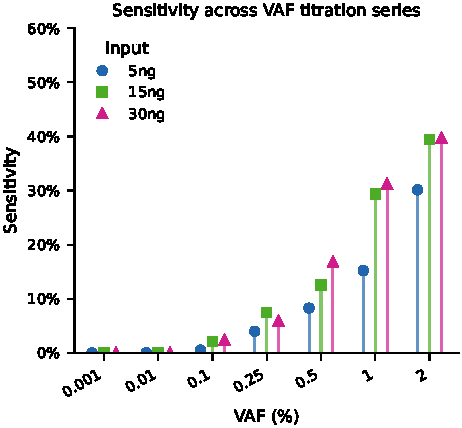
\includegraphics[width=\columnwidth]{figures/sensitivity_vs_vaf.pdf}
  \caption{Sensitivity by VAF and input mass. Each point shows sensitivity
    against the 375-variant truth set using 200K read pairs. Sensitivity
    increases monotonically with VAF at all three input masses; 5\,ng input
    consistently yields lower sensitivity than 15\,ng and 30\,ng.}
  \label{fig:sensitivity}
\end{figure}

\begin{figure}[t]
  \centering
  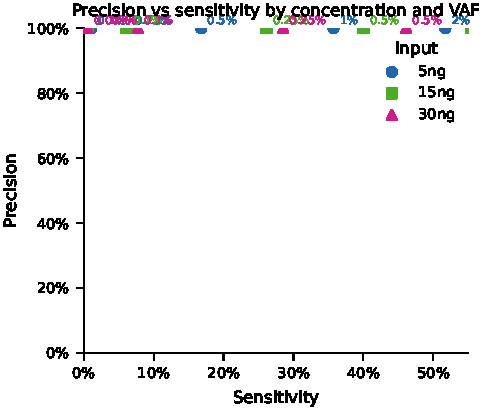
\includegraphics[width=\columnwidth]{figures/precision_recall.pdf}
  \caption{Precision vs sensitivity across all VAF/concentration combinations
    where at least one true positive was called. Each point is annotated with
    its VAF level. Precision is consistently above 0.37 wherever calls are
    made.}
  \label{fig:precision_recall}
\end{figure}

At 2\% VAF, the 15\,ng and 30\,ng samples achieve sensitivity of 39.5\% and
39.7\%, respectively, with precision of 0.60 and 0.60. The 5\,ng sample achieves
40.6\% sensitivity at 2\% VAF with precision of 0.62. The difference in
sensitivity between concentrations is most pronounced at intermediate VAF levels
(0.25\%–1\%), where lower input mass produces fewer starting molecules and
increases stochastic dropout.

Precision remains consistently high (0.37–0.62) wherever true positives are
called (Figure~\ref{fig:precision_recall}). False positives arise from two main
sources: (1) k-mer path artefacts where alternative paths through the de Bruijn
graph do not correspond to real variants, and (2) positions where the 100\,bp
target window covers a germline polymorphism not present in the reference
sequence used to build the allowlist.

% ── Negative control ──────────────────────────────────────────────────────────
\subsection{Negative control}

The 0\% VAF samples (no spiked variants) produced 23–48 PASS variant calls per
sample with 0–2 true positives. The very low true-positive count in the
negative control is an artefact of the scoring scheme: because some PASS calls
share genomic coordinates with truth variants by coincidence (e.g.\ a common
germline SNP at the same position), the scoring labels them as true positives
even though they are not somatic. The false positive count in the negative
control (26–42) gives an upper bound on the background artefact rate: roughly
30–45 per panel per sample at this sequencing depth.

% ── Runtime and memory ────────────────────────────────────────────────────────
\subsection{Runtime and memory}

Pipeline wall-clock time ranged from 3.5\,s to 21.4\,s per sample at 200K read
pairs on a single core. Peak RSS ranged from 450\,MB to 4.2\,GB, with most
samples under 600\,MB. Two outliers (30\,ng 0.1\% and 30\,ng 0.5\%) reached
4.2\,GB and 2.4\,GB respectively; these coincide with samples producing
particularly large de Bruijn graphs before path enumeration. Memory scaling is
a known issue discussed in Section~\ref{sec:evaluation}.
